Целью работы был перевод текста <<Методы и модели исследования уровня
профессиональных компетенций>>. 

Пример исходного текста:

\vspace{1.5em}

\small
\textbf{Модели распознавания образа уровня знаний.} Под образом уровня знаний понимаются обучаемые, принадлежащие к множеству (группе), знания которых по <<эталону уровня знаний>> отнесены к лингвистическим оценкам неудовлетворительно (D), удовлетворительно, хорошо, отлично. Под распознаванием образа уровня знаний понимается процедура принятия решения о принадлежности конкретного обучаемого к одному из указанных образов на основании сравнения его образовательных достижений при тестировании с характеристиками образа.

\textbf{Предметно -критериальная методика составления тестов} рассмотрена на основе работы <<Предметно-критериальная методика составления тестов>> Сысоевой Л. А., Толстоусовой В. Г. В каждом курсе есть ключевые моменты, особенно важные темы, без знания которых невозможно усвоение более сложного материала в процессе учебы или которые будут необходимы в работе по специальности. При автоматизированном тестировании можно учесть важность каких-либо разделов курса, увеличив долю вопросов по этим разделам в общем количестве вопросов. Но это не всегда удобно для составителя теста, потому что не всегда наиболее важные разделы содержат больше всего материала. Предлагаемая методика предусматривает учет таких параметров, как степень важности и объем изучаемого материала в разделах курса.

\textbf{Абсолютная временная шкала измерения знаний.} Данный подход был описано Крыловым Ю.Н. в работе <<Абсолютная временная шкала. Динамика результатов тестирования во времени>>. Этот подход подразумевает, что знания являются абсолютной субстанцией: они либо есть, либо их нет. По крайней мере, так считается в любой форме традиционного оценивания знаний - как на выпускных экзаменах в школах, так и на вступительных экзаменах в вузы. Поэтому интересно проанализировать возможности абсолютных шкал оценки и при переходе к измерению знаний на основе тестов. В данных исследованиях изучаются возможности так называемой <<абсолютной временной шкалы оценивания знаний>>. Формулируются ее принципы. Формулируются этапы последовательного перехода от традиционной формы экзаменов к тестовой форме этого подхода, на их основе - требования к созданию тестовых материалов этого подхода.

\textbf{Модель адаптивного тестового контроля.} Для её изучения были рассмотрены работы B.S.Bloom, R.M.Gagne, В.С.Аванесова. Процедура тестирования предполагает анализ ответов на последовательность тестовых заданий определенной сложности. Проведем аналогию с поведением поискового алгоритма оптимизации для некоторой гипотетической функция Y, максимум которой необходимо найти. В задачах оценивания по тестированию - это максимум функции уровня знаний. Реализация поискового алгоритма сводится к последовательному анализу локальной окрестности функционала Y, оценки градиента и выбора очередной области исследования. Если при оценке градиента имеют место помехи, то нельзя говорить о сходимости алгоритма. В обычном смысле он сходится вообще не будет, а будет <<блуждать>> вокруг области экстремума. Аналогично можно поступить в случае тестового контроля. Если ответ правильный, то предполагается, что уровень подготовки студента выше сложности предъявленной задачи и он способен решать задачи заданной сложности, в противном случае - неспособен. Это подобно оценке градиента некоторой гипотетической функции регрессии, в которой градиент сам является случайной величиной. 

\textbf{Автоматизированный контроль знаний по методике уточняющих вопросов} рассмотрен на основе работы И.Д. Рудинского и Е.В. Соловей <<Реализация алгоритмов прямого тестирования в интеллектуальной автоматизированной системе контроля знаний>>. Концепция базируется на автоматизации методики уточняющих вопросов, широко используемой в педагогической практике для выявления глубины знаний обучаемого. Относительная важность задаваемых вопросов определяется их весовыми коэффициентами, учитываемыми при подведении результатов тестирования. При подготовке к тестированию преподаватель имеет возможность определять или корректировать относительную важность каждого вопроса, устанавливать объем теста N, задавать время, отводимое экзаменуемому на демонстрацию своих знаний, и настраивать оценочную шкалу, по которой суммарный балл, набранный в ходе тестирования, переводится в итоговую оценку. В ходе автоматизированного тестирования экзаменуемому предъявляется конечное множество т.н. цепочек вопросов. Каждая цепочка представляет собой последовательность близких по тематике вопросов, формулируемых для уточнения знаний экзаменуемого. Очередной вопрос в цепочке задается только после получения ответа на предыдущий вопрос. В зависимости от стратегии тестирования, избираемой организатором контроля знаний, очередной вопрос в цепочке может предъявляться до первой ошибки (<<строгий>> преподаватель), либо экзаменуемому предоставляется возможность демонстрировать максимум знаний, отвечая на все вопросы данной тематической последовательности

\textbf{Дистанционная подготовка специалистов.}

Сегодня все чаще в системе образования используются термины <<новые технологии>>,
<<современные технологии>>. Чаще всего под ними понимается применение информационных технологий. Технологии, применяемые в системе образования должны быть перспективными, то есть нацеленными на использование технологий будущего.
Сегодня можно предположить следующие перспективные (активно развивающиеся              
сейчас) направления развития образования: 
\begin{enumerate}
  \item Дистанционное образование, в том числе дополнительное. 
  \item Виртуальные тренажеры. 
  \item Обучающие автоматизированные системы и игры. 
\end{enumerate}
В последнее время появление ряда научных и исследовательских работ, ориентированных на формирование систем согласованного управления рынком труда и сферы подготовки специалистов, говорит о формировании в обществе устойчивой тенденции к увеличению гибкости системы образования – появлению системы (институтов) дополнительного профессионального образования, в рамках которой и могут быть реализованы требования вариативности образовательных траекторий.

Дополнительное профессиональное образование можно отождествить с <<образованием взрослых>>, когда управляемость жизненной и карьерной траекториями осуществляется как со стороны обучающего (институтов обучения), так и самой личности. В последнем случае развитие навыков креативности не только способствует реализации внутреннего потенциала работника, но и является необходимым условием успешности его профессионального положения. 

Для удовлетворения потребностей рынка труда, а именно формирования у обучаемого (как будущего специалиста) набора лишь профессиональных знаний и умений, требуемых на производстве либо уже сегодня, либо в краткосрочной перспективе, подобная задача не является актуальной. Как следствие, значительно расширился рынок дополнительных образовательных услуг, отличительной особенностью которого является отказ от социально-культурной составляющей образования в пользу профессиональной составляющей и краткосрочность образовательных программ. Потребителями услуг этого рынка являются как работодатели, так и отдельные специалисты, появление которых на этом рынке предопределено предположительным характером требований и индивидуальных способностей (самооценка) при формировании ими своих трудовых отношений.

\newpage
\normalsize
Пример переведенного текста:
\vspace{1.5em}

\small

\textbf{The model of pattern recognition of the knowledge level.} The pattern of the knowledge level means trainees belonging to the group, which knowledge classified by ``standard knowledge level'' as linguistic grades: excellent (A), good (B), average (C) and difficulties (D). The pattern recognition of the knowledge level is a decision procedure about belonging of trainee to one of patterns based on comparison of its testing results and the characteristics of the pattern.

\textbf{The subject-criterial method of creating tests} was reviewed on the basis of work ``Subject-criterial method of test'' by Sysoeva L.A., Tolstousova V.G. Every course has its own key moments – especially important topics, without knowledge of which it is impossible to learn more difficult material, or specialty needs knowledge of those topics. In automatic testing it’s possible to take into account the importance of any topics by increasing the share of that topic’s questions in the total number of questions, but it isn’t always convenient for the test’s creator because sometimes important sections do not contain most of the material. The proposed method takes into consideration parameters such as the level of importance and the volume of learning material in sections of the course.

\textbf{The absolute time scale of knowledge measurement.} This approach was described by Krylov Y.N. in his work ``Absolute time scale. Dynamics of test results in time''. It assumes that knowledge is absolute substance: knowledge either exists or not. At least, that is considered to be in any form of traditional knowledge assessment: both at GCSE and at the entrance examinations. So it is interesting to analyze the possibilities of absolute scales of evaluation at the transition to the measurement of the knowledge-based tests. In these researches explored possibilities of so-called ``absolute time scale of knowledge evaluation'', formulated its principles; also formulated stages of sequential transition from traditional forms of exams to the test form of this approach, and the requirements for the creation of test materials based on these stages.

\textbf{Model of the adaptive control by tests.} To explore this model were considered works of Bloom B.S., Gagne R.M., Avanesov V.S. The testing procedure assumes the analysis of the answers to the sequence of tests of certain complexity. It is possible to draw an analogy with the behavior of search algorithm for a maximum of hypothetical function Y. In problems of estimation of testing it is the maximum of knowledge level function. The implementation of the search algorithm is reduced to the sequential analysis of the local neighborhood of functional Y, the gradient estimation and the selection of next area to explore. In conventional sense, it won’t converge, and will ``wander'' around the area of extreme. It’s possible to do likewise in the case of test control. If the answer is correct, the student’s preparation level is higher than complexity of problem and he is able to solve the problems of a given complexity, otherwise – he is unable. It is like an estimating of the gradient of the hypothetical regression function, in which the gradient is a random variable itself.

\textbf{Knowledge automatic control by the method of clarifying questions} was reviewed on the basis of work ``Implementation of direct testing algorithms in intellectual automated system of knowledge control'' by Rudinsky I.D. and Solovey E.V. The concept is based on automation of clarifying questions method, commonly used in teaching practice to indentify the depth of student’s knowledge. The relative importance of asked questions is determined by their weighting factors that are considered when summarizing the results of testing. When preparing for testing the teacher is able to determine or to correct the relative importance of each question, set the volume of test N, set the time allotted examinee to demonstrate their knowledge, set the scale by which the total points accumulated during the test are transferred to the final grade. During automatic testing examinee is presented finite set of so-called question chains. Each chain is a sequence of questions from similar subjects, which are formulated to clarify the examinee’s knowledge. Another question in the chain is given only after the answer to the previous question. Depending on the test strategy chosen by the organizer of the test, the next question in the chain will be given prior to the first error (``strict'' teacher), or the examinee can demonstrate the knowledge maximum by answering all question in the specific thematic chain.

\textbf{Specialists’ distance learning.} Today increasingly in the education system, the terms ``new technologies'' and ``modern technologies'' are used. Most often, they are understood as the use of information technologies. The technologies used in the education system must be promising, that means they must be targeted at the use of future technologies. Today, one can assume the following perspective (highly developing now) directions of development of education:
\begin{enumerate}
\item Remote education, including supplementary education.
\item Virtual training devices.
\item Educational games and automated systems. 
\end{enumerate}
Recently there have been several scientific and research works focused on the formation of labor market coherent management systems and training specialists. This suggests the formation of a stable tendency in society to increase the flexibility of education system, to create a system of supplementary professional education in which requirements of variability educational paths may be implemented.
Supplementary professional education can be identified with ``adult education'' when controllability of life and career carried out both by the trainer (or training institutions) and the personality. In the latter case, the development of skills of creativity not only helps employee to fulfill his inner potential, but is also a necessary condition for the success of his professional activities.
To meet the needs of the labor market, namely the formation of a trainee’s professional knowledge and skills required in the production either today or in the short term, such a problem is not relevant. As a consequence, the market of supplementary educational services has expanded significantly; the distinguish features of which are the rejection of the socio-cultural component of education for the benefit of professional component and the short educational programs. Consumers of this market are both employers and experts, whose appearance on this market is predetermined by conjectural character of requirements and individual abilities (self-esteem) at the formation of their employment relationship.

\newpage

\normalsize
Пример работы с рисунками:
\begin{figure}[h!]
  \center
  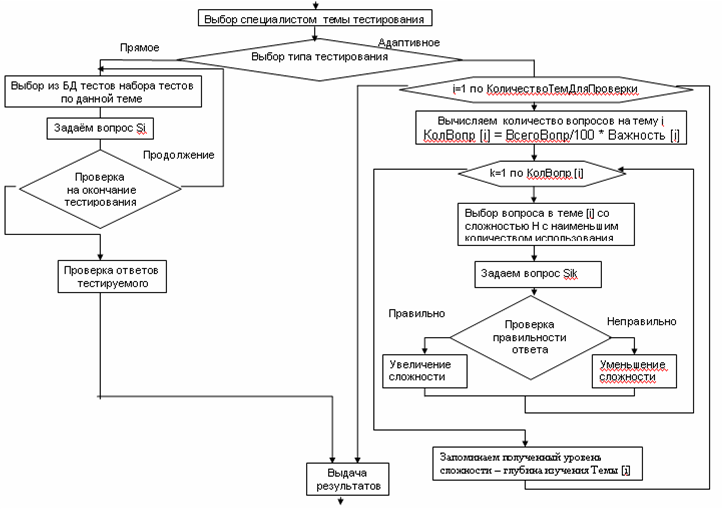
\includegraphics[width=.8\textwidth]{fig_11_rus} \\[.7em]
  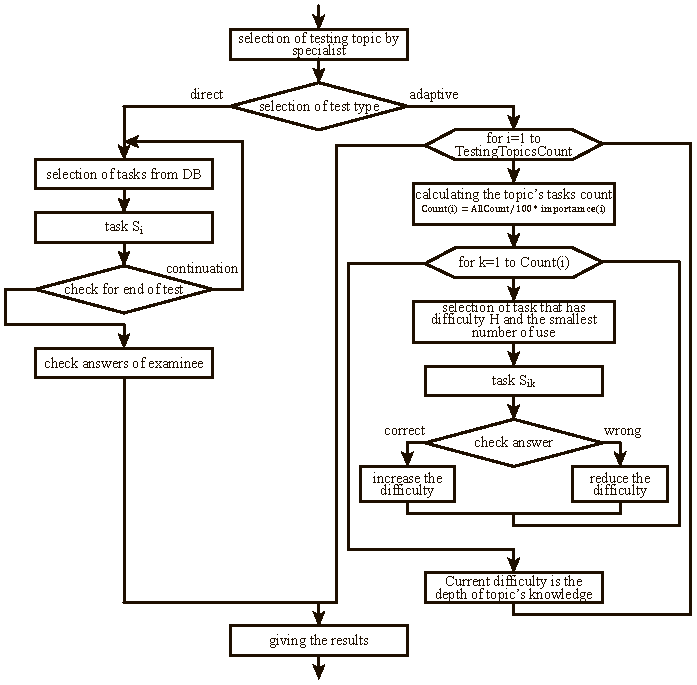
\includegraphics[width=.8\textwidth]{fig_11}
\end{figure}

\newpage

\begin{figure}[h!]
  \center
  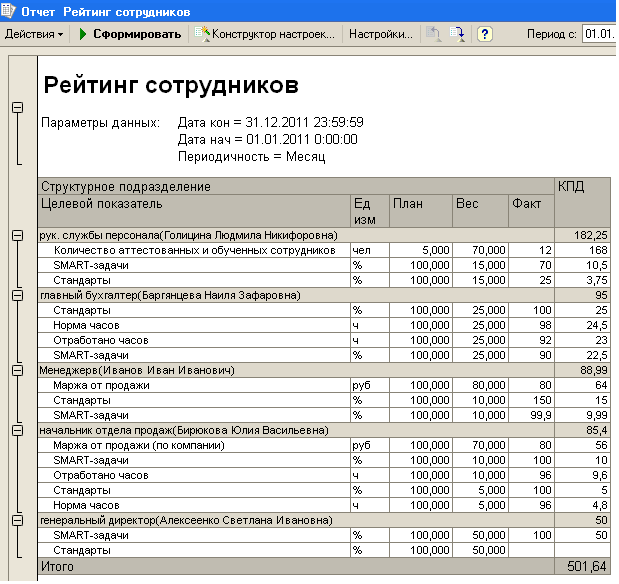
\includegraphics[width=.75\textwidth]{fig_45_rus} \\[.3em]
  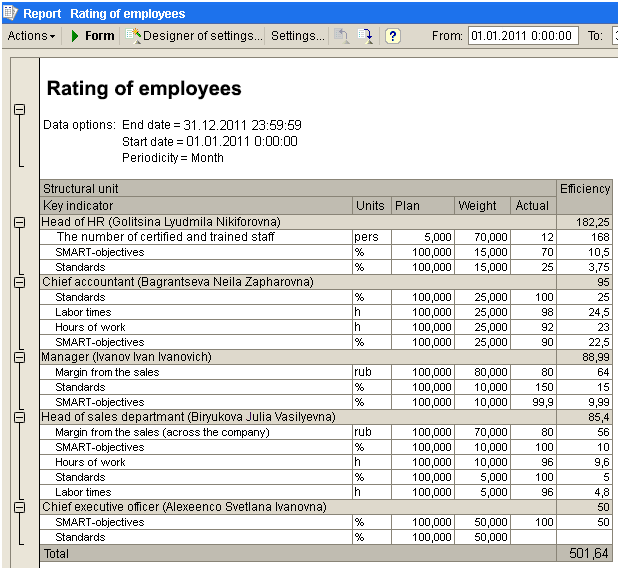
\includegraphics[width=.75\textwidth]{fig_45}
\end{figure}

Вывод: в результате выполнения семестровой работы данная статья была переведена.